\documentclass[12pt]{article}
\usepackage[a4paper, margin=2.5cm]{geometry}
\usepackage[utf8]{inputenc}
\usepackage[T1]{fontenc}
\usepackage{setspace}
\onehalfspacing
\usepackage{graphicx}
\usepackage{amsmath, amssymb}
\usepackage{booktabs}
\usepackage{caption}
\usepackage{float}
\usepackage{hyperref}
\usepackage{pgfplots}
\usetikzlibrary{intersections, patterns, decorations.markings, calc}

\title{Econometrics II -- Assignment 3:\\
A Dynamic Model for U.S. House Prices}
\date{Spring 2026}

\begin{document}

\maketitle
% ─────────────────────────────────────────────────────────────────────────────
\section{Introduction}
% ─────────────────────────────────────────────────────────────────────────────

This report examines whether U.S. house prices are linked to fundamentals through the long-run relationship
\begin{equation}
    h_t = \alpha + \beta_1 r_t + \beta_2 m_t,
\end{equation}
where $h_t$ is log house prices, $r_t$ is log rents, and $m_t$ is the mortgage rate. Using monthly data for 2012M1--2023M12, we test whether these variables are co-integrated and, if so, how deviations from equilibrium are corrected over time in a CVAR/VECM framework.
\newline
\newline
The empirical analysis first evaluates integration properties with ADF tests, then selects lag length in a VAR, determines co-integration rank with Johansen trace tests, and finally estimates the preferred CVAR specification with diagnostic checks before conclusions are drawn.
% ─────────────────────────────────────────────────────────────────────────────
\section{Description of the Data}
% ─────────────────────────────────────────────────────────────────────────────

The data come from \texttt{Assignment\_3.xlsx} and are based on FRED series for the S\&P/Case-Shiller U.S.
National Home Price Index, CPI rent of primary residence, and the 30-year fixed mortgage rate. The transformed variables are $h_t = \log(\text{HousePrice})$, $r_t = \log(\text{Rent})$, and $m_t = \text{MortgageRate}$. The effective sample contains 144 monthly observations.
\newline
\newline
Figure~\ref{fig:series_panel} shows that both $h_t$ and $r_t$ trend upward over the sample, while $m_t$ is much more cyclical and rises sharply in 2022--2023. This visual pattern is consistent with non-stationary behavior in the first two series and motivates a co-integration analysis rather than a stationary VAR in levels.

\begin{figure}[H]
	\centering
	
\includegraphics[width=0.7\textwidth]{figures/fig1_series_panel.pdf}
	\caption{Monthly series for $h_t$, $r_t$, and $m_t$, 2012M1--2023M12.}
	\label{fig:series_panel}
\end{figure}

\begin{table}[H]
\centering
\caption{Summary statistics for the analysis variables, 2012M1--2023M12.}
\label{tab:summary_stats}
\begin{tabular}{lrrrr}
\toprule
Variable & Mean & Std. Dev. & Min & Max \\
\midrule
h & 5.3108 & 0.2402 & 4.9165 & 5.7527 \\
r & 5.7511 & 0.1287 & 5.5501 & 6.0165 \\
m & 4.1642 & 1.0691 & 2.6800 & 7.6200 \\
\bottomrule
\end{tabular}
\end{table}


% ─────────────────────────────────────────────────────────────────────────────
\section{Econometric Theory}
% ─────────────────────────────────────────────────────────────────────────────

Let $X_t = (h_t, r_t, m_t)'$. Since the variables are treated as I(1), the natural framework is a VAR in levels rewritten as a co-integrated vector autoregression (CVAR):
\begin{equation}
    \Delta X_t = \Pi X_{t-1} + \Gamma_1 \Delta X_{t-1} + \cdots + \Gamma_{k-1}\Delta X_{t-k+1} + \mu + e_t,
\end{equation}
where $\Pi$ contains long-run information, $\Gamma_j$ capture short-run dynamics, and $e_t$ is a zero-mean innovation process. If $\Pi$ has reduced rank $r$, it can be factorized as
\[
\Pi = \alpha\beta',
\]
so the model becomes
\begin{equation}
    \Delta X_t = \alpha\beta'X_{t-1} + \Gamma_1 \Delta X_{t-1} + \cdots + \Gamma_{k-1}\Delta X_{t-k+1} + \mu + e_t.
    \label{eq:cvar}
\end{equation}
Here, $\beta$ contains the co-integrating vectors (long-run equilibria), while $\alpha$ contains adjustment coefficients measuring how each variable responds to disequilibrium. The constant is unrestricted, so the long-run relation may include a non-zero intercept.

The rank of $\Pi$ determines the system type. If $r=0$, there is no co-integration and the model reduces to a VAR in first differences. If $0<r<p$, there are $r$ stationary long-run relations among non-stationary variables. If $r=p$, the system is stationary in levels. In the present trivariate case ($p=3$), the key empirical question is therefore whether $r=0$ or $r\geq 1$.
\newline
\newline
Co-integration rank is determined by Johansen trace tests. For null hypothesis $H_0:r\leq r_0$ against $H_1:r>r_0$, the trace statistic is
\[
\mathrm{LR}_{\mathrm{trace}}(r_0) = -T\sum_{i=r_0+1}^{p}\ln(1-\hat{\lambda}_i),
\]
where $\hat{\lambda}_i$ are ordered generalized eigenvalues. The procedure is sequential, starting at $r_0=0$ and increasing until the first non-rejection.
\newline
With one co-integrating relation ($r=1$), normalization on house prices implies a long-run equation of the form
\[
h_t = c + \beta_r r_t + \beta_m m_t + u_t, \qquad u_t \sim I(0).
\]
This links directly to the user-cost benchmark: theory suggests $\beta_r=1$ and $\beta_m<0$. The first restriction corresponds to unit long-run rent elasticity, while the second reflects that higher mortgage rates increase user cost and reduce equilibrium house prices, ceteris paribus.
\newline
\newline
Finally, although co-integration is identified in a system, unit-root tests on individual variables are informative for model motivation. Hence ADF tests in levels and first differences are reported alongside the system evidence. Estimation of the CVAR is carried out by Gaussian maximum likelihood, and inference on rank and long-run restrictions is based on likelihood-ratio statistics, with misspecification checks used to evaluate whether the preferred dynamic specification is statistically adequate.

% ─────────────────────────────────────────────────────────────────────────────
\section{Empirical Analysis}
% ─────────────────────────────────────────────────────────────────────────────

\subsection{Integration Properties}

Table~\ref{tab:unit_root_tests} shows that the level series are clearly non-stationary: the ADF tests fail to reject a unit root for $h_t$, $r_t$, and $m_t$. In first differences, the null is rejected for $h_t$ and $m_t$, while $\Delta r_t$ is borderline at the 5\% level, which is not unusual in a short monthly sample with strong persistence. Taken together, the evidence is consistent with treating the three series as I(1) variables for co-integration analysis.

\begin{table}[H]
\centering
\caption{ADF unit-root tests (constant included).}
\label{tab:unit_root_tests}
\small
\setlength{\tabcolsep}{4pt}
\begin{tabular}{lrrr rrr}
\toprule
& \multicolumn{3}{c}{Level} & \multicolumn{3}{c}{First difference} \\
\cmidrule(lr){2-4}\cmidrule(lr){5-7}
Variable & Stat. & p-value & Lags & Stat. & p-value & Lags \\
\midrule
$h$ &  0.2679 & 0.9758 & 14 & -3.2160 & 0.0191 & 1 \\
$r$ &  1.7251 & 0.9982 & 12 & -2.6296 & 0.0870 & 8 \\
$m$ & -1.6255 & 0.4698 &  5 & -3.6555 & 0.0048 & 4 \\
\bottomrule
\end{tabular}
\normalsize
\end{table}


\subsection{Lag Selection}

The dynamic specification is chosen by estimating a VAR in levels and comparing lag-order criteria. Table~\ref{tab:lag_selection} shows that lag 4 minimizes both AIC and BIC, so the preferred VECM uses three lagged differences, that is, $k_{\Delta}=3$.

\begin{table}[H]
\centering
\caption{Lag-order selection criteria for VAR in levels (2012M1--2023M12).}
\label{tab:lag_selection}
\begin{tabular}{lrrr}
\toprule
Lag & AIC & BIC & HQIC \\
\midrule
0 & -10.3391 & -10.2736 & -10.3124 \\
1 & -29.0146 & -28.7525 & -28.9081 \\
2 & -30.7035 & -30.2449 & -30.5171 \\
3 & -30.9077 & -30.2525 & -30.6414 \\
4 & -31.1498 & -30.2980 & -30.8037 \\
5 & -31.1138 & -30.0655 & -30.6878 \\
6 & -31.0758 & -29.8309 & -30.5699 \\
7 & -31.0536 & -29.6122 & -30.4679 \\
8 & -31.0042 & -29.3662 & -30.3386 \\
9 & -31.0864 & -29.2519 & -30.3409 \\
10 & -31.0830 & -29.0519 & -30.2577 \\
11 & -31.0071 & -28.7795 & -30.1019 \\
12 & -30.9735 & -28.5494 & -29.9885 \\
\bottomrule
\end{tabular}
\end{table}


\subsection{Co-Integration Rank}

The Johansen trace test in Table~\ref{tab:johansen_trace} rejects the null of no co-integration, $r=0$, because the trace statistic 48.23 exceeds the 5\% critical value 29.80. The null $r\leq 1$ is not rejected, since the trace statistic 11.56 is below the 5\% critical value 15.49. Hence the preferred rank is $r=1$.
\newline
\newline
This implies one long-run equilibrium relation among house prices, rents, and mortgage rates. The fitted long-run component is shown in Figure~\ref{fig:coint_fit}, and the corresponding parameter estimates are reported in Table~\ref{tab:cvar_estimates}.

\begin{table}[H]
\centering
\caption{Johansen trace test. Sequential procedure rejects if trace stat. exceeds the 5\% critical value.}
\label{tab:johansen_trace}
\begin{tabular}{lrrrr}
\toprule
$H_0$ & Trace stat. & CV 90\% & CV 95\% & CV 99\% \\
\midrule
$r=0$ & 48.2266 & 27.0669 & 29.7961 & 35.4628 \\
$r\leq 1$ & 11.5648 & 13.4294 & 15.4943 & 19.9349 \\
$r\leq 2$ & 3.6207 & 2.7055 & 3.8415 & 6.6349 \\
\bottomrule
\end{tabular}
\end{table}


\begin{table}[H]
\centering
\caption{Preferred CVAR (k=4, unrestricted constant, rank 1). Normalised on $h_t$. Std. err.\ from VECM ML.}
\label{tab:cvar_estimates}
\begin{tabular}{lrr}
\toprule
Parameter & Estimate & Std. err. \\
\midrule
$\beta_r$ (rent elasticity) & 1.4918 & 0.0467 \\
$\beta_m$ (mortgage coef.) & 0.0085 & 0.0068 \\
$\alpha_h$ & 0.0156 & 0.0049 \\
$\alpha_r$ & 0.0091 & 0.0018 \\
$\alpha_m$ & 0.3958 & 0.5380 \\
\bottomrule
\end{tabular}
\end{table}


\begin{figure}[H]
	\centering
	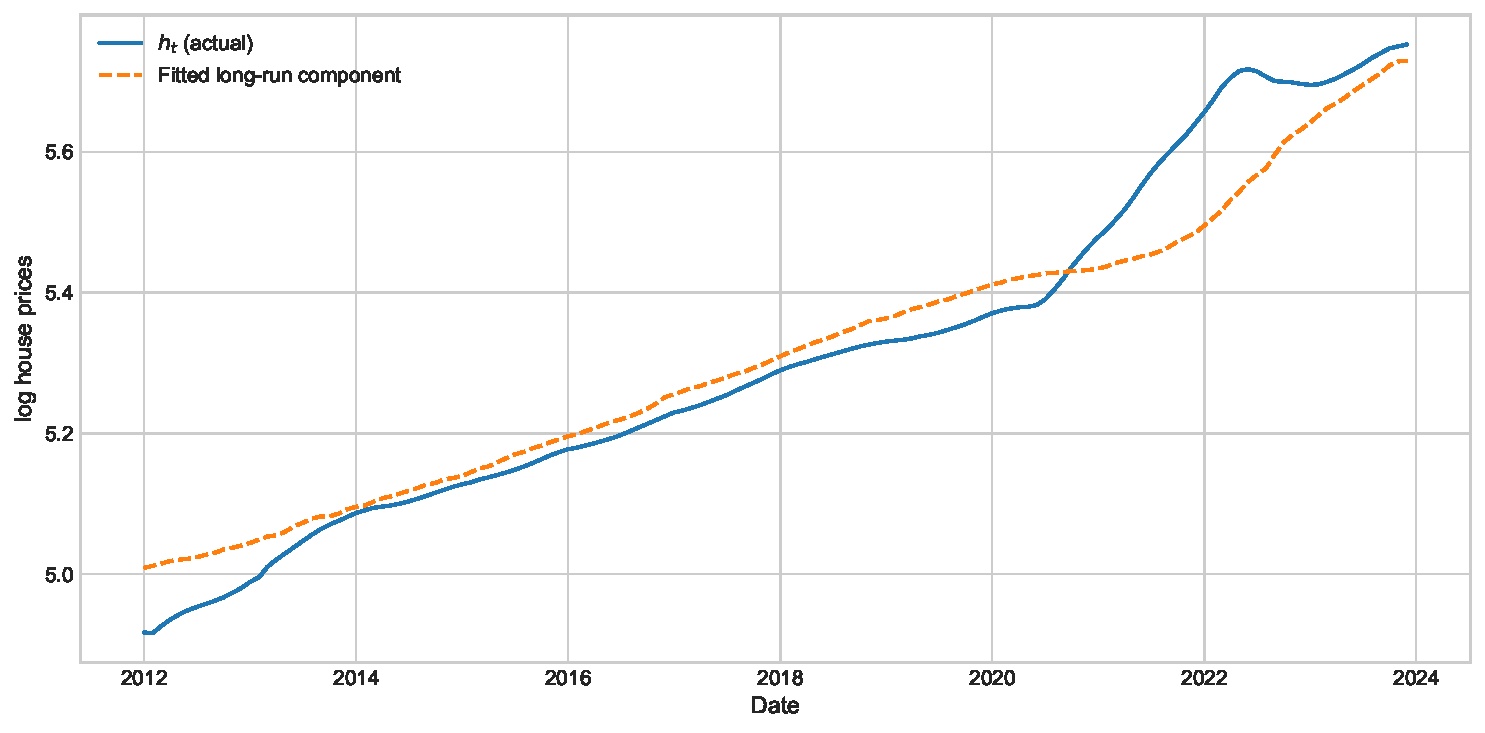
\includegraphics[width=0.9\textwidth]{figures/fig2_cointegration_fit.pdf}
	\caption{Actual $h_t$ and fitted long-run component from the preferred CVAR.}
	\label{fig:coint_fit}
\end{figure}

\subsection{Preferred CVAR and Interpretation}

Normalizing the co-integrating vector on house prices gives the estimated long-run relation
\begin{equation}
	h_t = \hat c + 1.4918\, r_t + 0.0085\, m_t.
\end{equation}
The rent coefficient is positive and larger than one, so the strict unit-elasticity restriction $\beta_1=1$ is not supported by the point estimate. The mortgage-rate coefficient is also positive, which is not the sign predicted by the strict user-cost model. In other words, the data support a stable long-run link, but not the exact theoretical sign pattern imposed by the simplest version of the model.
\newline
The adjustment coefficients indicate how equilibrium is restored after a deviation from the long-run relation. The loading on mortgage rates, $\alpha_m = 0.3958$, is much larger in absolute terms than the loadings on house prices and rents, $\alpha_h = 0.0156$ and $\alpha_r = 0.0091$. This suggests that the mortgage-rate equation absorbs most of the short-run correction, while house prices and rents adjust only weakly.

Figure~\ref{fig:coint_fit} shows that the fitted equilibrium component captures the low-frequency movement in house prices, even though short-run fluctuations remain substantial.

\subsection{Misspecification Diagnostics}

The residual diagnostics in Table~\ref{tab:diagnostics} are mixed. The Portmanteau whiteness test has $p=0.3012$, so there is no evidence of remaining serial correlation in the preferred specification. By contrast, the Jarque-Bera test strongly rejects normality, and the ARCH LM test for mortgage-rate residuals rejects homoskedasticity at the 5\% level.
\newline
These diagnostics matter for interpretation. The co-integration result is not driven by omitted residual autocorrelation, but the non-normality and ARCH effects indicate that the Gaussian likelihood approximation is imperfect, most likely because the post-2021 interest-rate shock is unusually large relative to the rest of the sample.

\begin{table}[H]
\centering
\caption{Misspecification diagnostics for the preferred CVAR specification.}
\label{tab:diagnostics}
\begin{tabular}{lrr}
\toprule
Test & Statistic & p-value \\
\midrule
Whiteness (Portmanteau) & 83.9923 & 0.3012 \\
Normality (Jarque--Bera) & 391.7401 & 0.0000 \\
ARCH LM (h) & 19.1037 & 0.0861 \\
ARCH LM (r) & 6.4636 & 0.8909 \\
ARCH LM (m) & 23.7053 & 0.0223 \\
\bottomrule
\end{tabular}
\end{table}


% ─────────────────────────────────────────────────────────────────────────────
\section{Discussion}

The empirical evidence supports one co-integrating relation between house prices, rents, and mortgage rates in the 2012M1--2023M12 sample. However, the economic content of the relation is only partly aligned with the textbook user-cost model. The rent elasticity is above one rather than equal to one, and the mortgage-rate coefficient has the wrong sign in the estimated long-run relation. This suggests that the simplified model omits relevant channels, such as risk premia, financing conditions, or other time-varying user-cost components.
\newline
The diagnostics also show that the sample is not well behaved in a Gaussian sense. The combination of non-normal residuals and ARCH effects points to crisis-like observations and a major regime shift in the interest-rate environment. For that reason, the estimated equilibrium relation should be read as a useful average long-run approximation rather than a structural law. A natural robustness extension would be to repeat the exercise on a longer sample that includes the pre-2012 housing boom and crisis period.

% ─────────────────────────────────────────────────────────────────────────────
\section{Conclusion}
% ─────────────────────────────────────────────────────────────────────────────

The preferred VAR lag length is 4, the Johansen trace test selects rank 1, and the corresponding CVAR therefore implies one long-run equilibrium relation among house prices, rents, and mortgage rates. The fitted relation is economically meaningful in the sense that house prices and rents move together over time, but the point estimates do not fully support the strict user-cost benchmark: the rent elasticity exceeds one and the mortgage-rate coefficient is positive. Equilibrium adjustment is mainly carried by the mortgage-rate equation, while residual autocorrelation is not a concern. The main caveat is non-normality and ARCH, which makes the sample sensitive to the post-2021 rate shock and motivates a robustness check on a longer sample.

\bigskip
\noindent\textbf{References}

\noindent Anundsen, A.K. (2019). Detecting Imbalances in House Prices: What Goes Up Must Come Down? \textit{The Scandinavian Journal of Economics}, 121(4), 1587--1619.

\noindent Johansen, S. (1995). \textit{Likelihood-Based Inference in Cointegrated Vector Autoregressive Models}. Oxford University Press.

\end{document}